% ! TEX root = ./Incompressible_Flow_over_Airfoils.tex

\tikzset{every picture/.style={line width=0.75pt}} %set default line width to 0.75pt        

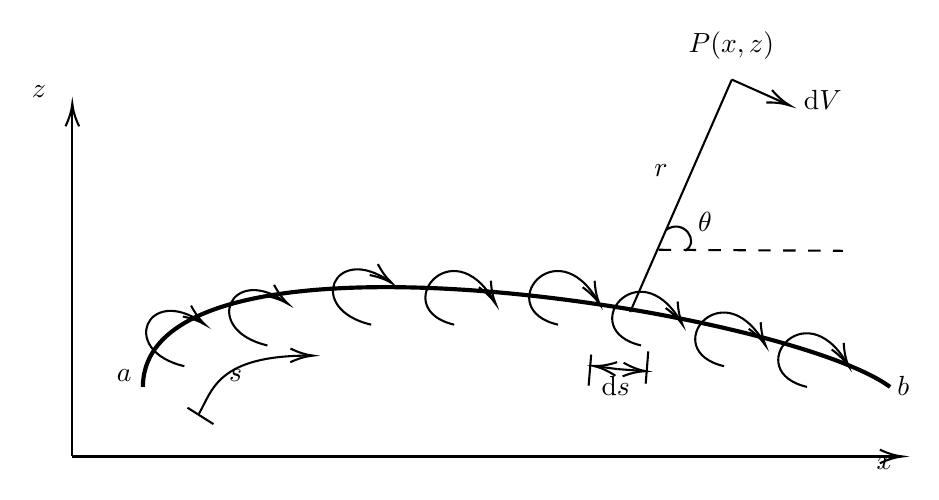
\begin{tikzpicture}[x=0.75pt,y=0.75pt,yscale=-1,xscale=1]
%uncomment if require: \path (0,285); %set diagram left start at 0, and has height of 285

%Curve Lines [id:da8763652678817189] 
\draw [line width=1.5]    (104,206.5) .. controls (104.51,119.91) and (414,169.5) .. (464,206.5) ;
%Curve Lines [id:da4750021580535706] 
\draw    (124,196.5) .. controls (92,189.03) and (106.07,156.9) .. (132.77,175.61) ;
\draw [shift={(134,176.5)}, rotate = 216.83] [color={rgb, 255:red, 0; green, 0; blue, 0 }  ][line width=0.75]    (10.93,-3.29) .. controls (6.95,-1.4) and (3.31,-0.3) .. (0,0) .. controls (3.31,0.3) and (6.95,1.4) .. (10.93,3.29)   ;
%Curve Lines [id:da2895808384347458] 
\draw    (164,186.5) .. controls (132,179.03) and (146.07,146.9) .. (172.77,165.61) ;
\draw [shift={(174,166.5)}, rotate = 216.83] [color={rgb, 255:red, 0; green, 0; blue, 0 }  ][line width=0.75]    (10.93,-3.29) .. controls (6.95,-1.4) and (3.31,-0.3) .. (0,0) .. controls (3.31,0.3) and (6.95,1.4) .. (10.93,3.29)   ;
%Curve Lines [id:da7153231460572151] 
\draw    (214,176.5) .. controls (182,169.03) and (196.07,136.9) .. (222.77,155.61) ;
\draw [shift={(224,156.5)}, rotate = 216.83] [color={rgb, 255:red, 0; green, 0; blue, 0 }  ][line width=0.75]    (10.93,-3.29) .. controls (6.95,-1.4) and (3.31,-0.3) .. (0,0) .. controls (3.31,0.3) and (6.95,1.4) .. (10.93,3.29)   ;
%Curve Lines [id:da9877697377632966] 
\draw    (254,176.5) .. controls (222,169.03) and (252.56,130.11) .. (273.07,164.86) ;
\draw [shift={(274,166.5)}, rotate = 241.4] [color={rgb, 255:red, 0; green, 0; blue, 0 }  ][line width=0.75]    (10.93,-3.29) .. controls (6.95,-1.4) and (3.31,-0.3) .. (0,0) .. controls (3.31,0.3) and (6.95,1.4) .. (10.93,3.29)   ;
%Curve Lines [id:da6202187083118886] 
\draw    (304,176.5) .. controls (272,169.03) and (302.56,130.11) .. (323.07,164.86) ;
\draw [shift={(324,166.5)}, rotate = 241.4] [color={rgb, 255:red, 0; green, 0; blue, 0 }  ][line width=0.75]    (10.93,-3.29) .. controls (6.95,-1.4) and (3.31,-0.3) .. (0,0) .. controls (3.31,0.3) and (6.95,1.4) .. (10.93,3.29)   ;
%Curve Lines [id:da8336758488674814] 
\draw    (344,186.5) .. controls (312,179.03) and (342.56,140.11) .. (363.07,174.86) ;
\draw [shift={(364,176.5)}, rotate = 241.4] [color={rgb, 255:red, 0; green, 0; blue, 0 }  ][line width=0.75]    (10.93,-3.29) .. controls (6.95,-1.4) and (3.31,-0.3) .. (0,0) .. controls (3.31,0.3) and (6.95,1.4) .. (10.93,3.29)   ;
%Curve Lines [id:da8897778956265143] 
\draw    (384,196.5) .. controls (352,189.03) and (382.56,150.11) .. (403.07,184.86) ;
\draw [shift={(404,186.5)}, rotate = 241.4] [color={rgb, 255:red, 0; green, 0; blue, 0 }  ][line width=0.75]    (10.93,-3.29) .. controls (6.95,-1.4) and (3.31,-0.3) .. (0,0) .. controls (3.31,0.3) and (6.95,1.4) .. (10.93,3.29)   ;
%Curve Lines [id:da04487167241342771] 
\draw    (424,206.5) .. controls (392,199.03) and (422.56,160.11) .. (443.07,194.86) ;
\draw [shift={(444,196.5)}, rotate = 241.4] [color={rgb, 255:red, 0; green, 0; blue, 0 }  ][line width=0.75]    (10.93,-3.29) .. controls (6.95,-1.4) and (3.31,-0.3) .. (0,0) .. controls (3.31,0.3) and (6.95,1.4) .. (10.93,3.29)   ;
%Straight Lines [id:da5621055060339388] 
\draw    (125.5,216.5) -- (138.01,224.41) ;
%Curve Lines [id:da3596797142445818] 
\draw    (131.01,219.41) .. controls (137.45,208.52) and (139.47,191.26) .. (184.63,191.4) ;
\draw [shift={(186.01,191.41)}, rotate = 180.62] [color={rgb, 255:red, 0; green, 0; blue, 0 }  ][line width=0.75]    (10.93,-3.29) .. controls (6.95,-1.4) and (3.31,-0.3) .. (0,0) .. controls (3.31,0.3) and (6.95,1.4) .. (10.93,3.29)   ;
%Straight Lines [id:da4909959828720716] 
\draw    (347.5,189.41) -- (346.26,204.91) ;
%Straight Lines [id:da5091055511160192] 
\draw    (318.76,205.91) -- (320,190.91) ;
%Straight Lines [id:da5213093595184453] 
\draw    (332.76,197.91) -- (344.27,198.77) ;
\draw [shift={(346.26,198.91)}, rotate = 184.24] [color={rgb, 255:red, 0; green, 0; blue, 0 }  ][line width=0.75]    (10.93,-3.29) .. controls (6.95,-1.4) and (3.31,-0.3) .. (0,0) .. controls (3.31,0.3) and (6.95,1.4) .. (10.93,3.29)   ;
%Straight Lines [id:da04498336011734372] 
\draw    (332.76,197.91) -- (323.24,196.67) ;
\draw [shift={(321.26,196.41)}, rotate = 7.43] [color={rgb, 255:red, 0; green, 0; blue, 0 }  ][line width=0.75]    (10.93,-3.29) .. controls (6.95,-1.4) and (3.31,-0.3) .. (0,0) .. controls (3.31,0.3) and (6.95,1.4) .. (10.93,3.29)   ;
%Straight Lines [id:da31365051851853876] 
\draw    (338.76,170.41) -- (387.76,58.41) ;
%Straight Lines [id:da29570303575193213] 
\draw  [dash pattern={on 4.5pt off 4.5pt}]  (352.5,140.41) -- (368.26,140.5) -- (441.26,140.91) ;
%Curve Lines [id:da3186708293732772] 
\draw    (356,130.91) .. controls (364.26,124.91) and (372.76,136.41) .. (365.26,140.91) ;
%Straight Lines [id:da09450810625839368] 
\draw    (387.76,58.41) -- (413.94,70.1) ;
\draw [shift={(415.76,70.91)}, rotate = 204.06] [color={rgb, 255:red, 0; green, 0; blue, 0 }  ][line width=0.75]    (10.93,-3.29) .. controls (6.95,-1.4) and (3.31,-0.3) .. (0,0) .. controls (3.31,0.3) and (6.95,1.4) .. (10.93,3.29)   ;
%Straight Lines [id:da5222357770732207] 
\draw    (70,240) -- (70,72) ;
\draw [shift={(70,70)}, rotate = 90] [color={rgb, 255:red, 0; green, 0; blue, 0 }  ][line width=0.75]    (10.93,-3.29) .. controls (6.95,-1.4) and (3.31,-0.3) .. (0,0) .. controls (3.31,0.3) and (6.95,1.4) .. (10.93,3.29)   ;
%Straight Lines [id:da5641055148269973] 
\draw    (70,240) -- (468,240) ;
\draw [shift={(470,240)}, rotate = 180] [color={rgb, 255:red, 0; green, 0; blue, 0 }  ][line width=0.75]    (10.93,-3.29) .. controls (6.95,-1.4) and (3.31,-0.3) .. (0,0) .. controls (3.31,0.3) and (6.95,1.4) .. (10.93,3.29)   ;

% Text Node
\draw (90,196.5) node [anchor=north west][inner sep=0.75pt]    {$a$};
% Text Node
\draw (144,196.5) node [anchor=north west][inner sep=0.75pt]    {$s$};
% Text Node
\draw (466,200) node [anchor=north west][inner sep=0.75pt]    {$b$};
% Text Node
\draw (323.5,199.91) node [anchor=north west][inner sep=0.75pt]    {$\mathrm{d}s$};
% Text Node
\draw (349,97.91) node [anchor=north west][inner sep=0.75pt]    {$r$};
% Text Node
\draw (370,120.91) node [anchor=north west][inner sep=0.75pt]    {$\theta $};
% Text Node
\draw (365.5,33.91) node [anchor=north west][inner sep=0.75pt]    {$P(x,z)$};
% Text Node
\draw (421,61.91) node [anchor=north west][inner sep=0.75pt]    {$\mathrm{d}V$};
% Text Node
\draw (49,60) node [anchor=north west][inner sep=0.75pt]    {$z$};
% Text Node
\draw (456,239) node [anchor=north west][inner sep=0.75pt]    {$x$};


\end{tikzpicture}
